\documentclass[11pt,a4paper]{article}
%\documentclass[11pt,a4paper,twoside]{article}
\usepackage[utf8]{inputenc}
\usepackage[french]{babel}
\usepackage[T1]{fontenc}

\usepackage{amsmath}
\usepackage{amsfonts}
\usepackage{amssymb}

\newcommand{\TitreMatiere}{Architecture des Ordinateurs}
\newcommand{\TitreSeance}{Autres Codages Binaires}
\newcommand{\NumeroTD}{Gray \& BCD}
\newcommand{\DateCours}{Octobre 2023}
\newcommand{\AnneeScolaire}{2023-2024}
\newcommand{\Organisation}{EPITA}
\newcommand{\NomAuteurA}{Fabrice BOISSIER}
\newcommand{\MailAuteurA}{fabrice.boissier@epita.fr}
\newcommand{\NomAuteurB}{ }
\newcommand{\MailAuteurB}{ }
\newcommand{\DocKeywords}{Architecture}
\newcommand{\DocLangue}{fr} % "en", "fr", ...

\usepackage{MetalCourseBooklet}

% Babel ne traduit pas toujours bien les tableaux et autres
\renewcommand*\frenchfigurename{%
    {\scshape Figure}%
}
\renewcommand*\frenchtablename{%
    {\scshape Tableau}%
}

% Ne pas afficher le numéro de la légende sur tableaux et figures
\captionsetup{format=sanslabel}


\usepackage{xlop}  % Ajout des jolies divisions posées :   \opdiv{25}{7}  \opidiv{25}{7}
%\usepackage{pstricks}  % style pour xlop

\begin{document}

\EncadreTitre

\bigskip


%\begin{center}
%\begin{tabular}{p{5cm} p{11cm}}
%\textbf{Commandes étudiées :} & \texttt{sh}, \texttt{bash}, \texttt{man}, \texttt{ls}, \texttt{mkdir}, \texttt{touch}, \texttt{chmod}, \texttt{mv}, \texttt{rm}, \texttt{rmdir}, \texttt{cat}, \texttt{file}, \texttt{which}, \texttt{which}\\
%
%\textbf{Builtins étudiées :} & \texttt{pwd}, \texttt{cd}, \texttt{exit}, \texttt{logout}, \texttt{echo}, \texttt{umask}, \texttt{type}, \texttt{>}, \texttt{>{}>}, \texttt{<}, \texttt{<{}<}, \texttt{|}\\
%
%\textbf{Notions étudiées :} & Shell, Manuels, Fichiers, Répertoires, Droits, Redirections\\
%\end{tabular}
%\end{center}

\bigskip


Ce document a pour objectif de vous familiariser avec les autres codages binaires utilisés dans l'industrie : le code Gray et le code BCD.

\bigskip

Tout comme le format binaire classique que vous avez déjà vu, ces codages permettent de représenter des nombres entiers en binaire (avec des 0 et des 1), mais dans des formats différents.
Ils sont fréquemment utilisés dans certains contextes tels que l'électronique, ou pour aider à la résolution de problèmes logiques.

\bigskip

Encore une fois : une donnée binaire n'est qu'une donnée, c'est son interprétation qui est importante afin de comprendre l'information qu'elle véhicule ainsi que pour savoir quelles opérations il est possible d'effectuer avec.
Par exemple, l'opération d'incrémentation en binaire classique propage une retenue de la droite vers la gauche.
Néanmoins, lorsque l'on utilise d'autres formats, incrémenter ou décrémenter ne s'effectue pas de la même manière.
Ainsi, il faut choisir les opérateurs adaptés au format de la donnée manipulée, ou éventuellement d'abord la transformer en binaire classique, effectuer l'opération désirée, puis re-transformer le résultat dans le format initial.


\vfillFirst

\vfillLast

%\bigskip

%%%%%%%%%%%%%%%%%%%%%%%%%%%%%%%%%%%%%%%%%%%%%%%%%%%%%%%%%%%%%%%%%%%%%%%%%
%%%%%%%%%%%%%%%%%%%%%%%%%%%%%%%%%%%%%%%%%%%%%%%%%%%%%%%%%%%%%%%%%%%%%%%%%
%%%%%%%%%%%%%%%%%%%%%%%%%%%%%%%%%%%%%%%%%%%%%%%%%%%%%%%%%%%%%%%%%%%%%%%%%
%%%%%%%%%%%%%%%%%%%%%%%%%%%%%%%%%%%%%%%%%%%%%%%%%%%%%%%%%%%%%%%%%%%%%%%%%

\section{Code Gray}

\bigskip

Le code Gray est un codage utilisé dans certains instruments, en particulier dans des capteurs de positions utilisant des angles, mais aussi dans les tableaux de Karnaugh pour les circuits logiques (qui serons abordés dans un autre cours).

\medskip

L'idée du codage Gray est de ne modifier qu'un seul bit entre chaque incrémentation (on retrouve ce principe dans le code Baudot anciennement utilisé dans les télégraphes).
Par exemple, entre $ 143 $ et $ 144 $, en représentation classique il faut modifier 5 bits, tandis qu'en code Gray, il n'y a qu'un seul bit qui varie :

\medskip

\begin{table}[!ht]
  \centering
  \begin{minipage}{0.47\textwidth}
    \centering

Codage binaire classique

\smallskip

\bf
\begin{tabular}{ | C{1.5cm} | c c c c  m{0.25cm} c c c c | }
\hline
     &   &   &   &   & &   &   &   &   \\
143  & 1 & 0 & 0 & 0 & & 1 & 1 & 1 & 1 \\
     &   &   &   &   & &   &   &   &   \\
\hline
     &   &   &   &   & &   &   &   &   \\
144  & 1 & 0 & 0 & 1 & & 0 & 0 & 0 & 0 \\
     &   &   &   &   & &   &   &   &   \\
\hline
\end{tabular}
%
\begin{tabular}{   C{1.5cm}   c c c c  m{0.25cm} c c c c }
     & \phantom{1}  & \phantom{1} & \phantom{1} & $\uparrow$ & & $\uparrow$ & $\uparrow$ & $\uparrow$ & $\uparrow$ \\
\end{tabular}

  \end{minipage}
  \hfillx
  \begin{minipage}{0.47\textwidth}
    \centering

Code Gray

\smallskip

\bf
\begin{tabular}{ | C{1.5cm} | c c c c  m{0.25cm} c c c c | }
\hline
     &   &   &   &   & &   &   &   &   \\
143  & 1 & 1 & 0 & 0 & & 1 & 0 & 0 & 0 \\
     &   &   &   &   & &   &   &   &   \\
\hline
     &   &   &   &   & &   &   &   &   \\
144  & 1 & 1 & 0 & 1 & & 1 & 0 & 0 & 0 \\
     &   &   &   &   & &   &   &   &   \\
\hline
\end{tabular}
%
\begin{tabular}{   C{1.5cm}   c c c c  m{0.25cm} c c c c }
     & \phantom{1}  & \phantom{1} & \phantom{1} & $\uparrow$ & & \phantom{1} & \phantom{1} & \phantom{1} & \phantom{1} \\
\end{tabular}

  \end{minipage}
%  \caption{Algorithme de la somme des N premiers entiers}
%  \label{somme-n-premiers-entiers}
\end{table}


Incrémenter en code Gray ne respecte donc absolument pas le principe de propagation de retenue de la droite vers la gauche.
Il n'est donc pas possible d'additionner ou soustraire de la manière habituelle des nombres codés dans le format Gray.

\bigskip

Plusieurs méthodes pour \og construire \fg{} le Gray code sont possibles.
La plus connue est la méthode dite du \textit{code binaire réfléchi}, qui impose de construire le code depuis $ 0 $.
Parmi les autres méthodes, il existe plusieurs formules qui permettent de passer du code binaire classique au code Gray et réciproquement.


%\bigskip
\clearpage

%%%%%%%%%%%%%%%%%%%%%%%%%%%%%%%%%

\subsection{Code Binaire Réfléchi}

Le code binaire réfléchi est une technique visuelle pour énumérer toutes les valeurs du code Gray.
On écrit chaque nombre sur une ligne à la fois, en commençant tout d'abord par $ 0 $ et $ 1 $, puis, une fois que l'on a consommé tous les emplacements/bits de position possible, on recopie les lignes déjà écrites en appliquant un miroir tout en ajoutant un $ 1 $ dans la position suivante.


\begin{table}[!ht]
  \centering
  \begin{minipage}{0.30\textwidth}
    \centering

\begin{tabular}{ | c | c c c c | }
\hline
0  & & & & \tikzmarknode{t1A}{0} \\
1  & & & & 1 \\
\hline
2  & & & 1 & 1 \\
3  & & & 1 & \tikzmarknode{t1B}{0} \\
\hline
\end{tabular}

\vfillFirst

\vfillLast

\begin{tabular}{ | c | c c c c |}
\hline
0  & & & 0 & 0 \\
1  & & & 0 & 1 \\
2  & & & 1 & \tikzmarknode{t2A}{1} \\
3  & & & 1 & 0 \\
\hline
4  & & 1 & 1 & 0 \\
5  & & 1 & 1 & \tikzmarknode{t2B}{1} \\
6  & & 1 & 0 & 1 \\
7  & & 1 & 0 & 0 \\
\hline
\end{tabular}

\tikz[remember picture, overlay]{\draw[latex-latex,black,line width=0.75mm] ([yshift=0.1em,xshift=1em]t1A.east) to[bend left] ([yshift=0.1em,xshift=1em]t1B.east);}

\tikz[remember picture, overlay]{\draw[latex-latex,black,line width=0.75mm] ([yshift=0.1em,xshift=1em]t2A.east) to[bend left] ([yshift=0.1em,xshift=1em]t2B.east);}

  \end{minipage}
  \hfillx
  \begin{minipage}{0.25\textwidth}
    \centering

\begin{tabular}{ | c | c c c c | }
\hline
0  &   &   &   & {\color{gray} 0} \\
\hline
1  &   &   &   & 1 \\
\hline
2  &   &   & 1 & 1 \\
3  &   &   & 1 & 0 \\
\hline
4  &   & 1 & 1 & 0 \\
5  &   & 1 & 1 & 1 \\
6  &   & 1 & 0 & 1 \\
7  &   & 1 & 0 & 0 \\
\hline
8  & 1 & 1 & 0 & 0 \\
9  & 1 & 1 & 0 & 1 \\
10 & 1 & 1 & 1 & 1 \\
11 & 1 & 1 & 1 & 0 \\
12 & 1 & 0 & 1 & 0 \\
13 & 1 & 0 & 1 & 1 \\
14 & 1 & 0 & 0 & 1 \\
15 & 1 & 0 & 0 & 0 \\
\hline
\end{tabular}

  \end{minipage}
  \hfillx
  \begin{minipage}{0.35\textwidth}
    \centering

\begin{tabular}{ | c | c c c c | c c c c |}
\hline
 & \multicolumn{4}{c|}{Code Gray} & \multicolumn{4}{c|}{Code Binaire} \\
\hline
0  & 0 & 0 & 0 & 0 &   0 & 0 & 0 & 0 \\
\hline
1  & 0 & 0 & 0 & 1 &   0 & 0 & 0 & 1 \\
\hline
2  & 0 & 0 & 1 & 1 &   0 & 0 & 1 & 0 \\
3  & 0 & 0 & 1 & 0 &   0 & 0 & 1 & 1 \\
\hline
4  & 0 & 1 & 1 & 0 &   0 & 1 & 0 & 0 \\
5  & 0 & 1 & 1 & 1 &   0 & 1 & 0 & 1 \\
6  & 0 & 1 & 0 & 1 &   0 & 1 & 1 & 0 \\
7  & 0 & 1 & 0 & 0 &   0 & 1 & 1 & 1 \\
\hline
8  & 1 & 1 & 0 & 0 &   1 & 0 & 0 & 0 \\
9  & 1 & 1 & 0 & 1 &   1 & 0 & 0 & 1 \\
10 & 1 & 1 & 1 & 1 &   1 & 0 & 1 & 0 \\
11 & 1 & 1 & 1 & 0 &   1 & 0 & 1 & 1 \\
12 & 1 & 0 & 1 & 0 &   1 & 1 & 0 & 0 \\
13 & 1 & 0 & 1 & 1 &   1 & 1 & 0 & 1 \\
14 & 1 & 0 & 0 & 1 &   1 & 1 & 1 & 0 \\
15 & 1 & 0 & 0 & 0 &   1 & 1 & 1 & 1 \\
\hline
\end{tabular}

  \end{minipage}
%  \caption{Algorithme de la somme des N premiers entiers}
%  \label{somme-n-premiers-entiers}
\end{table}

On remarque que les plus grandes valeurs avant chaque puissance de 2 (c'est-à-dire $ 3 $, $ 7 $, $ 15 $, ...) ne sont plus constituées exclusivement de 1, mais sont au contraire constituées d'un 1 suivi de 0 exclusivement.

%\bigskip
\medskip
%\smallskip

Une des raisons de ce fonctionnement est que le code Gray se transpose parfaitement dans des capteurs d'angles.
En effet, les transitions qui ne modifient qu'un seul bit avec l'effet miroir correspondent en réalité à une roue graduée où chaque anneau représente un bit précis :

\begin{table}[!ht]
  \centering
  \begin{minipage}{0.45\textwidth}
    \centering

  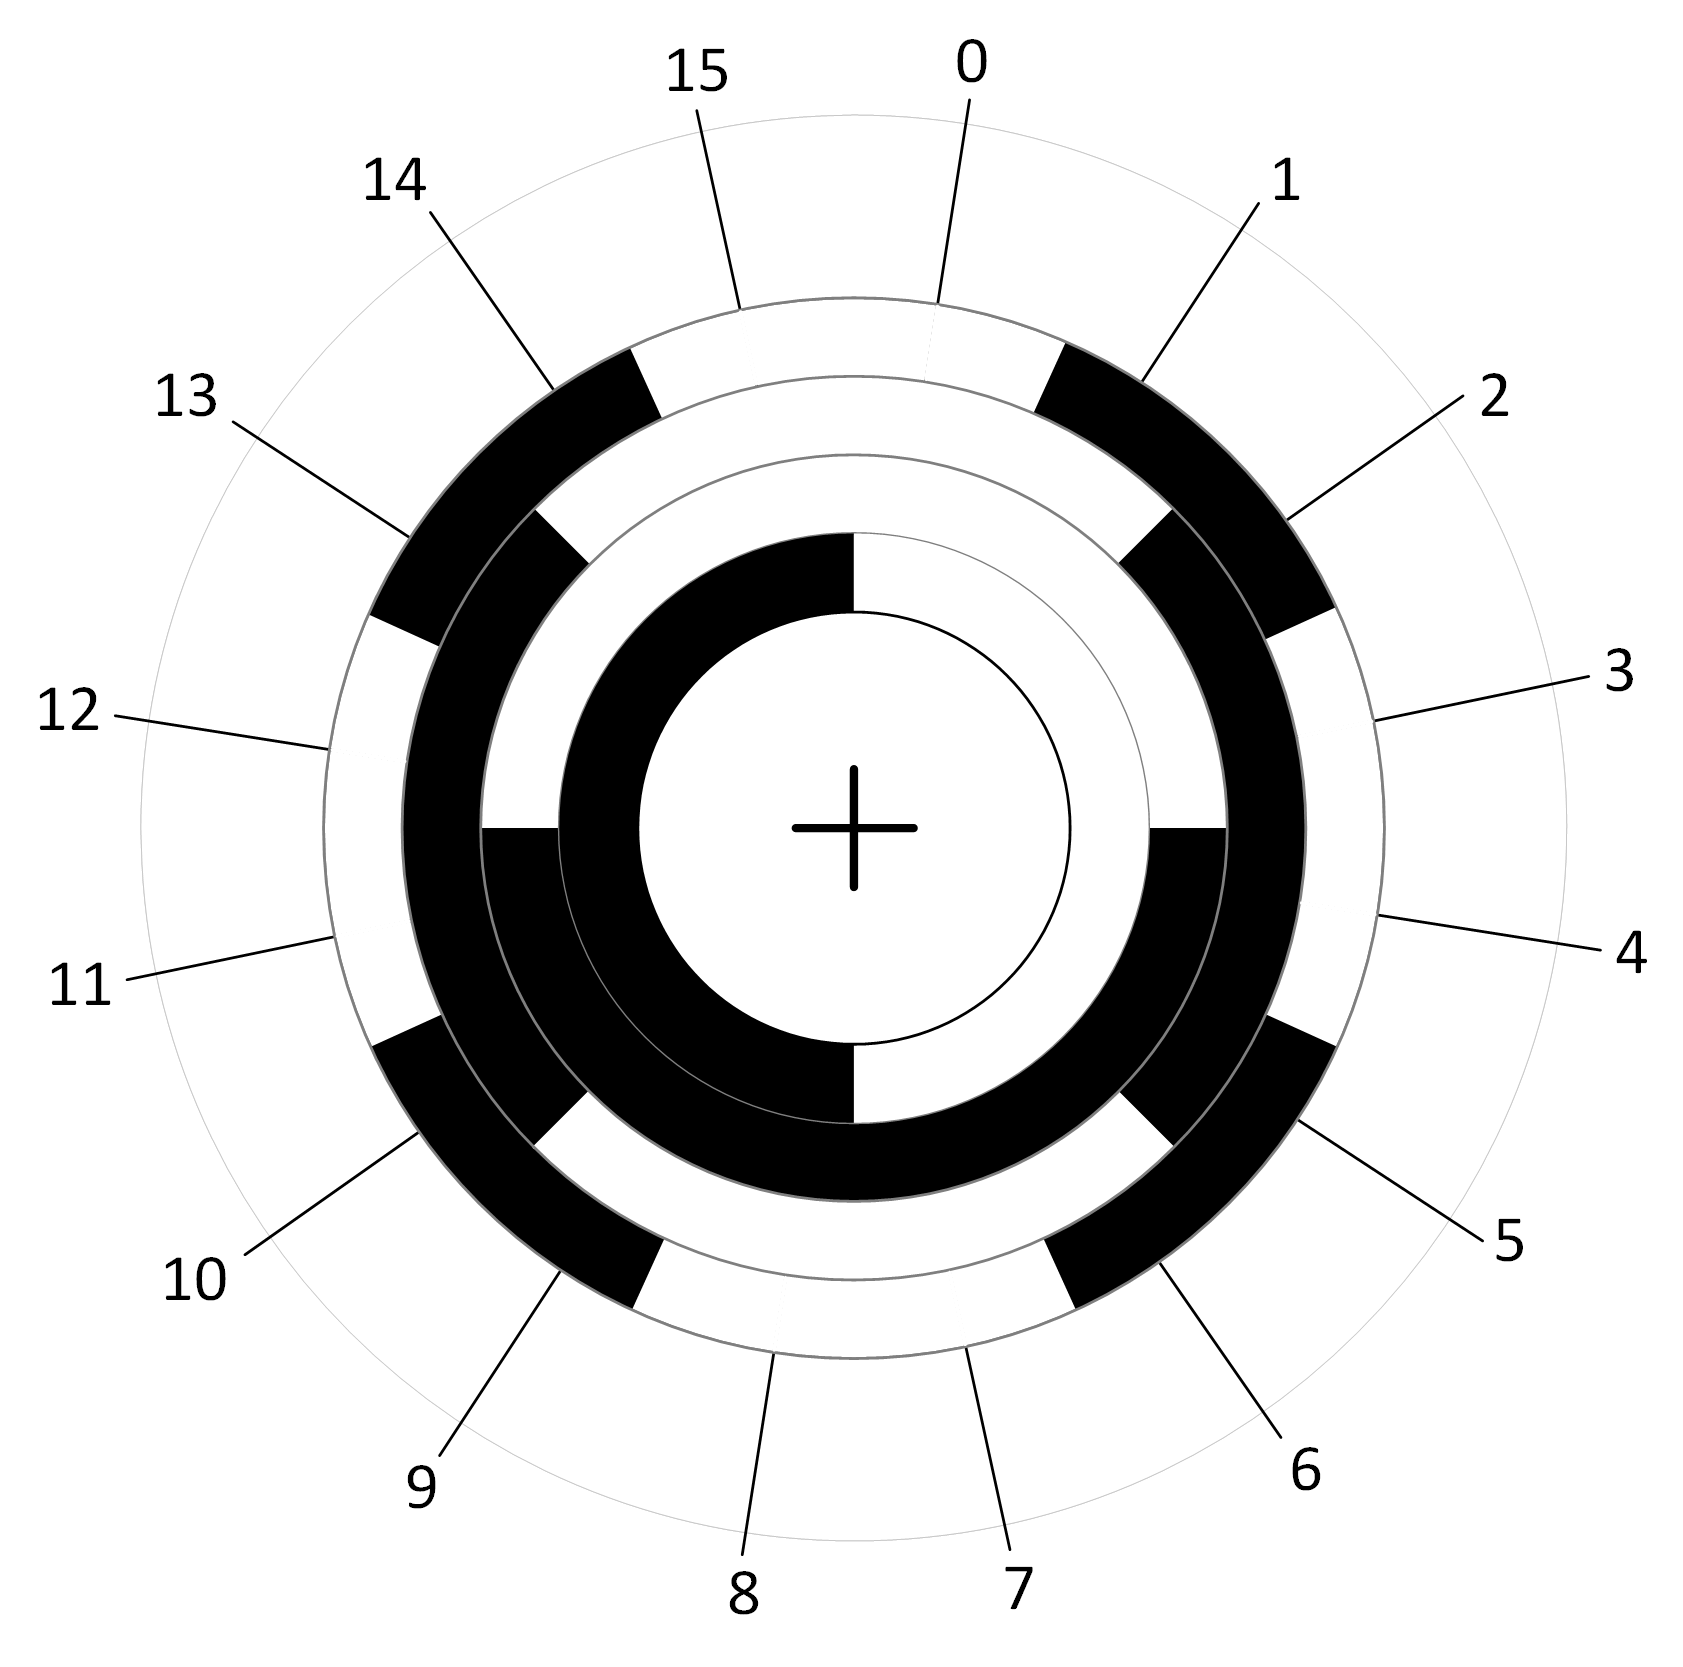
\includegraphics[scale=0.35]{img/BCD_Gray/Roue_Codeuse_Gray_4bits.png}

  \phantom{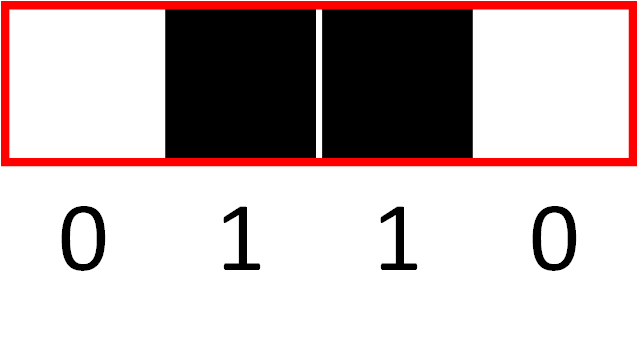
\includegraphics[scale=0.24]{img/BCD_Gray/Code_Gray_4.png}}

  Roue codeuse Gray sur 4 bits

%  \includegraphics[scale=0.5]{img/BCD_Gray/EXTERNAL_UNAUTHORIZED/roue-codeuse-gray.png}
%
%  Roue codeuse Gray sur 4 bits
%
%  \textit{(Image extraite du site~\href{https://www.positron-libre.com/cours/electronique/logique-combinatoire/codage-information/code-gray.php}{Positron-Libre})}
%
%  \phantom{Texte.}

  \end{minipage}
  \hfillx
  \begin{minipage}{0.45\textwidth}
    \centering

  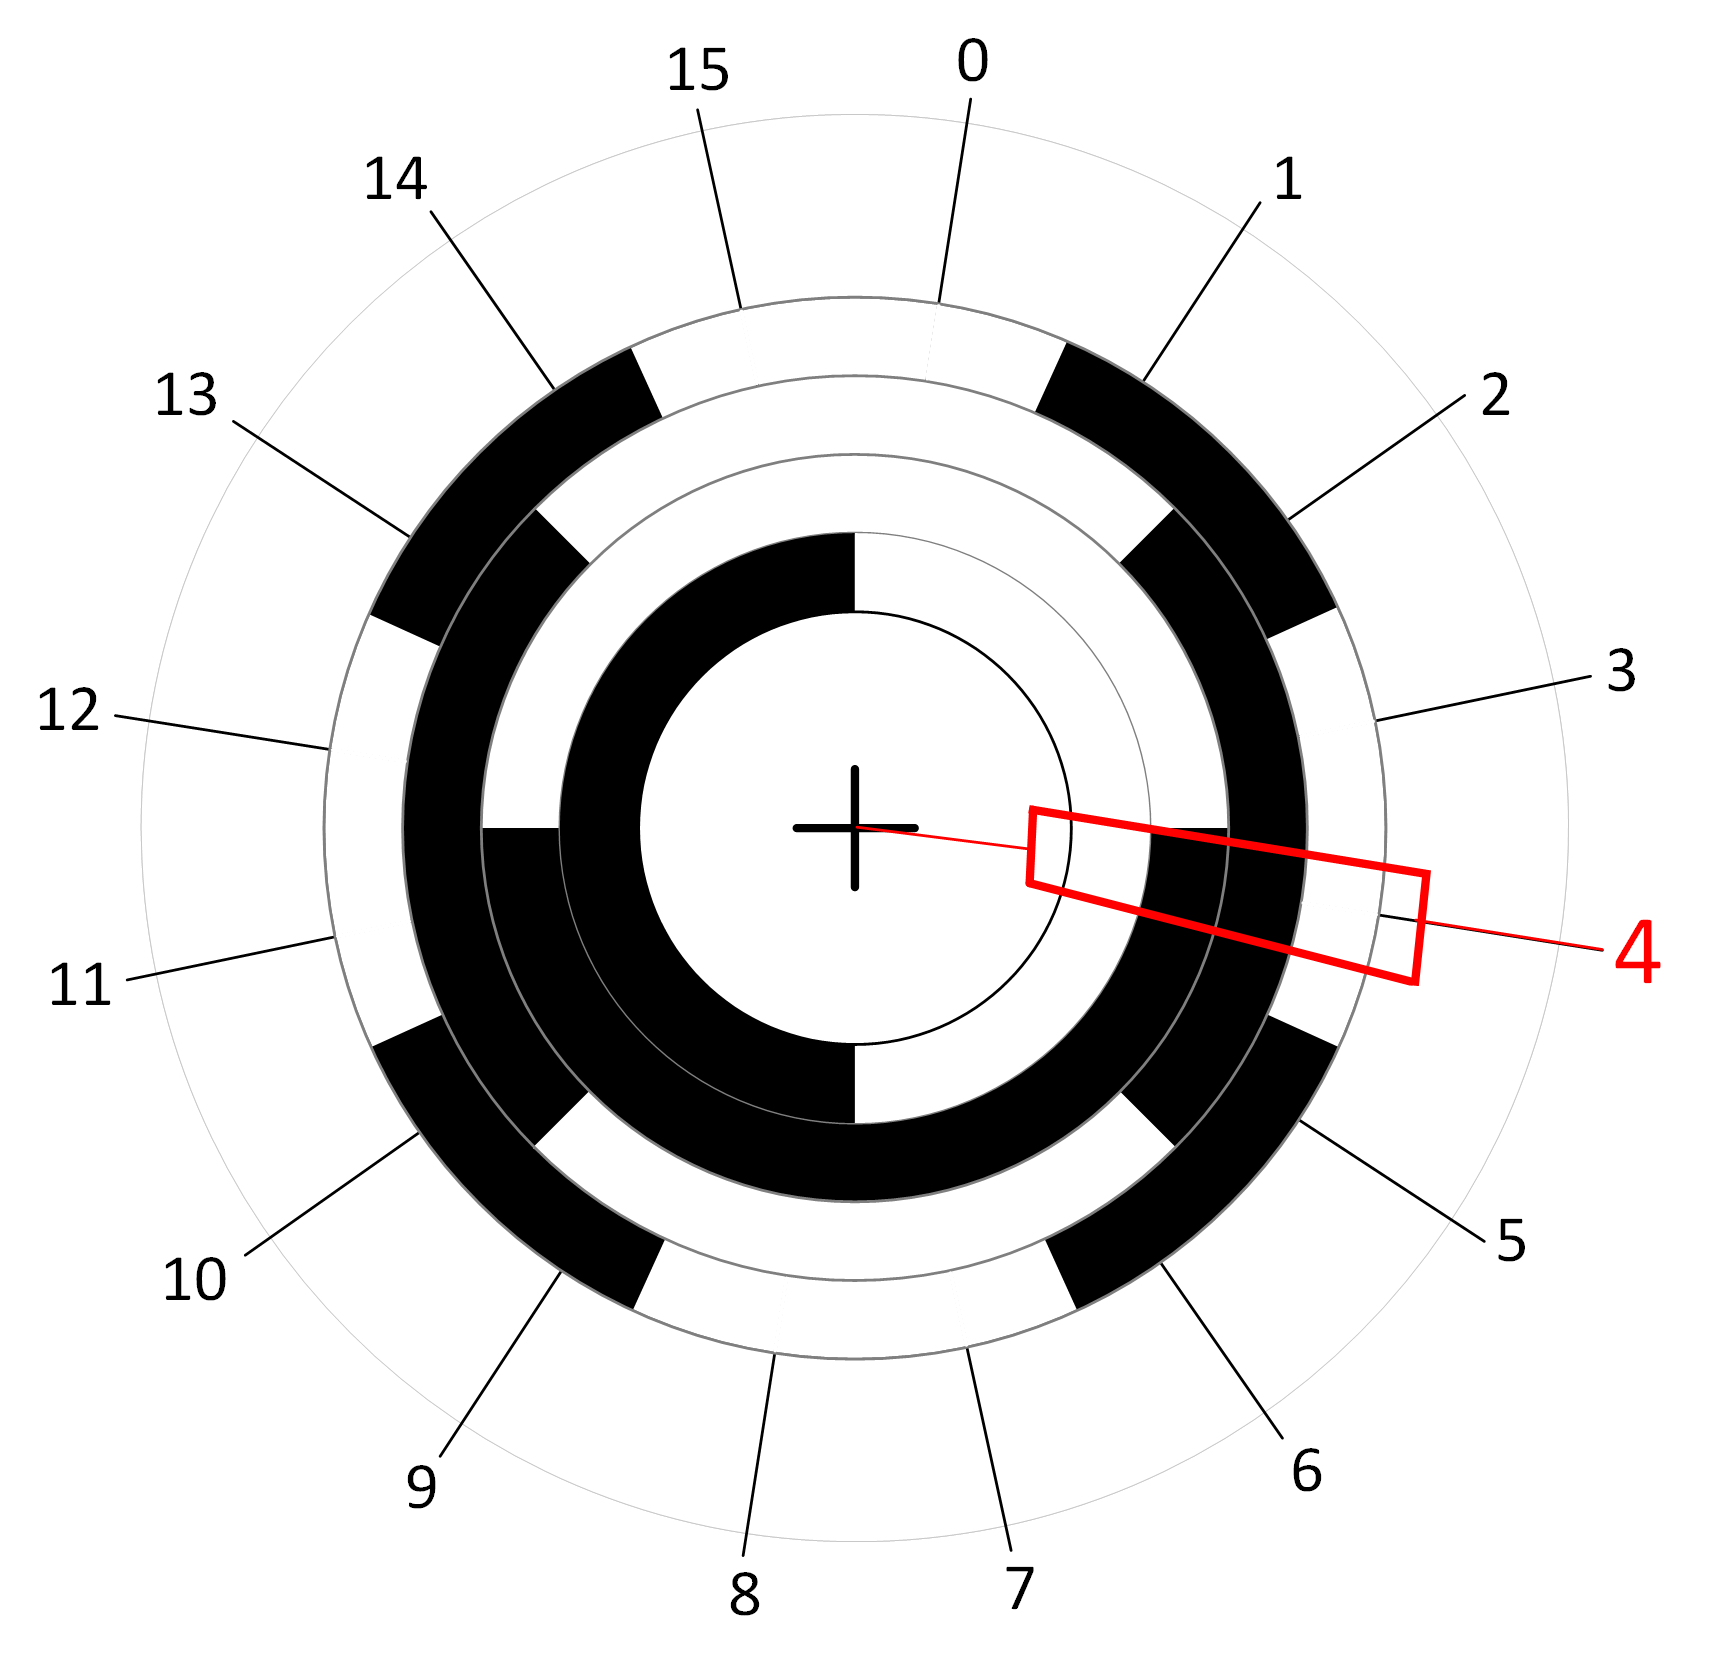
\includegraphics[scale=0.35]{img/BCD_Gray/Roue_Codeuse_Gray_4bits_Example_4.png}

  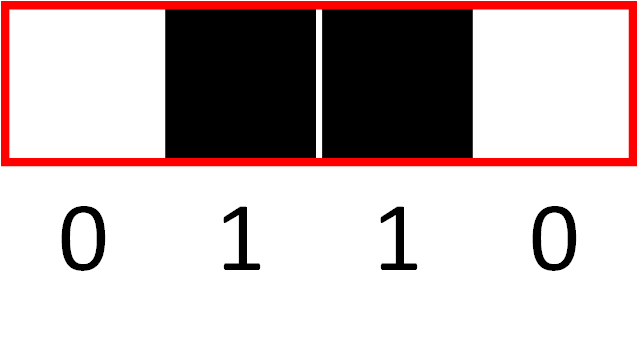
\includegraphics[scale=0.24]{img/BCD_Gray/Code_Gray_4.png}

   Codage Gray du nombre \og 4 \fg{} : $ \text{\%} \, 0110 $


%  \includegraphics[scale=0.68]{img/BCD_Gray/EXTERNAL_UNAUTHORIZED/roue-codeuse-gray-4.png}
%
%   Codage Gray du nombre \og 4 \fg{} : $ \text{\%} \, 0110 $
%
%   Une zone noire correspond à un 1, \\ et une zone blanche à un 0

  \end{minipage}
\end{table}

Ainsi, la position d'un objet sur le cadran peut être détectée et comprise au travers d'un nombre au format Gray.
On peut également en déduire l'angle depuis la position codant la valeur 0.

Chaque anneau représentant un bit : plus on voudra gagner en précision sur la position, plus il faudra ajouter d'anneaux extérieurs, et donc élargir le format de la représentation binaire.


\bigskip

%%%%%%%%%%%%%%%%%%%%%%%%%%%%%%%%%

\subsection{Binaire vers Gray : Formule mathématique}

Une première formule permet de passer du code binaire classique au code Gray.
C'est même la méthode la plus simple pour passer de n'importe quel nombre vers du code Gray lorsque vous maîtrisez le binaire classique.

\begin{equation*}
\text{Code Gray}(N) = \frac{N \oplus 2N}{2} = \frac{N \; \textsc{xor} \; 2N}{2}
\end{equation*}

\medskip

La formule est relativement simple :
\begin{enumerate}
\item on prend un nombre que l'on convertit en binaire
\item on calcule son double (c'est-à-dire qu'on le décale vers la gauche en ajoutant un 0),
\item on effectue l'opération \textsc{xor} sur les deux,
\item on divise le résultat par 2 (c'est-à-dire que l'on décale vers la droite en effaçant le nombre après la virgule).
\end{enumerate}




\begin{table}[!ht]
  \centering
  \begin{minipage}{0.80\textwidth}

Prenons $ 143 $ comme exemple :
\begin{enumerate}
\item $ 143 = \text{\%} 1000 \; 1111 $
\item $ 143 \times 2 = \text{\%} 1000 \; 1111 \times 2 = \text{\%} 1000 \; 1111 \; 0 = \text{\%} 1 \; 0001 \; 1110 = 286 $
\item $ 143 \oplus 286 = \text{\%} 1000 \; 1111 \oplus \text{\%} 1 \; 0001 \; 1110 = \text{\%} 1 \; 1001 \; 0001 $

\begin{tabular}{c m{0.05cm} c m{0.05cm} c c c c m{0.05cm} c c c c}
         & &   & & 1 & 0 & 0 & 0 & & 1 & 1 & 1 & 1 \\
$\oplus$ & & 1 & & 0 & 0 & 0 & 1 & & 1 & 1 & 1 & 0 \\
\hline
         & & 1 & & 1 & 0 & 0 & 1 & & 0 & 0 & 0 & 1 \\
\end{tabular}

\item $ \frac{143 \oplus 286}{2} = \text{\%} 1 \; 1001 \; 0001 \div 2 = \text{\%} 1100 \; 1000,1 \Rightarrow \text{\%} \underline{1100 \; 1000} $
\end{enumerate}

  \end{minipage}
  \hfillx
  \begin{minipage}{0.18\textwidth}
    \centering

    \begin{tabular}{|c|c|c|}
        \hline
        A & B & \TTBF{XOR} \\
        \hline
        0 & 0 & 0 \\
        \hline
        0 & 1 & 1 \\
        \hline
        1 & 0 & 1 \\
        \hline
        1 & 1 & 0 \\
        \hline
    \end{tabular}

  \end{minipage}
\end{table}


\bigskip

%%%%%%%%%%%%%%%%%%%%%%%%%%%%%%%%%

\subsection{Binaire vers Gray : Formule bit à bit}

Une autre formule plus technique existe et consiste à déduire l'état de chaque bit entre le code Gray et son équivalent binaire.
Cette technique est l'application directe en électronique de la formule précédente.

\bigskip

Dans la notation qui suit, les $ B_{n} $ correspondent au $ N^{\text{ième}} $ bit de la valeur binaire classique, en partant de la puissance $ 0 $.
La notation $ G_{n} $ correspond au $ N^{\text{ième}} $ bit de la valeur en code Gray.
Concrètement, $ 13_{10} $ équivaut à $ \text{\%} 1101 $ en binaire classique, ce qui indique que le bit 2 (donc $ B_{2} $) est à 0, tandis que les bits 4, 3, et 1 (donc $ B_{4} \, B_{3} \, B_{1} $) sont à 1.


\begin{table}[!ht]
  \centering
  \begin{minipage}{0.45\textwidth}
    \centering
Binaire classique

\bigskip

\begin{tabular}{ c  | c | c | c | c | }
13                    & $B_{4}$ & $B_{3}$ & $B_{2}$ & $B_{1}$ \\
\hline
$ \text{\%} \, 1101 $ & 1 & 1 & 0 & 1 \\
\end{tabular}

  \end{minipage}
  \hfillx
  \begin{minipage}{0.45\textwidth}
    \centering
Code Gray

\bigskip

\begin{tabular}{ c  | c | c | c | c | }
13                    & $G_{4}$ & $G_{3}$ & $G_{2}$ & $G_{1}$ \\
\hline
$ \text{\%} \, 1011 $ & 1 & 0 & 1 & 1 \\
\end{tabular}

  \end{minipage}
\end{table}

\smallskip

On notera également que ce que l'on appelle le \textit{LSB} en anglais (\textit{Least Significant Bit}) correspond en français au \textit{bit de poids faible}, c'est-à-dire le numéro de bit qui contient la puissance de 2 la plus petite, donc le bit codant $ 2^{0} $.

On peut également trouver dans la littérature la mention du \textit{MSB} en anglais (\textit{Most Significant Bit}) qui correspond en français au \textit{bit de poids fort}, c'est-à-dire le bit contenant la puissance de 2 la plus grande dans le format choisi.

Ainsi, sur 12 bits, le \textit{LSB} sera $ B_{1} $ qui correspond à $ 2^{0} $, et le \textit{MSB} sera $ B_{12} $ qui correspond à $ 2^{11} $.
Sur 8 bits, le \textit{LSB} sera le même ($ B_{1} $ correspondant à $ 2^{0} $), et le \textit{MSB} sera $ B_{8} $ qui correspond à $ 2^{7} $.

\medskip

Ces mentions \textit{LSB} et \textit{MSB} permettent de savoir dans quel sens lire les valeurs (de gauche à droite ou de droite à gauche).

\bigskip
\bigskip

On peut déduire un nombre au format Gray à partir de son équivalent au format binaire classique grâce à une formule calculant l'état de chaque bit.
Il s'agit en réalité de la formule représentant le circuit d'un composant électronique dédié à la traduction de nombres au format binaire classique vers le format Gray.
Ce circuit est l'application réelle de la formule mathématique vu précédemment.

\begin{equation*}
G_{n} = B_{n} \oplus B_{n + 1} = B_{n} \; \text{\textsc{xor}} \; B_{n + 1}
\end{equation*}

\medskip

Ainsi, on déduit l'état de $ G_{1} $ à partir de l'état de $ B_{1} $ et $ B_{2} $.

\bigskip
\bigskip

Essayons avec $ 13 $ , c'est-à-dire $ \text{\%} \, 1101 $ en binaire classique :

\smallskip

\begin{table}[!ht]
  \centering
  \begin{minipage}{0.40\textwidth}

\begin{itemize}
\item $ G_{1} = B_{1} \oplus B_{2} = 1 \oplus 0 = 1 $
\item $ G_{2} = B_{2} \oplus B_{3} = 0 \oplus 1 = 1 $
\item $ G_{3} = B_{3} \oplus B_{4} = 1 \oplus 1 = 0 $
\item $ G_{4} = B_{4} \oplus \textcolor{gray}{B_{5}} = 1 \oplus \textcolor{gray}{0} = 1 $
\end{itemize}

  \end{minipage}
  \hfillx
  \begin{minipage}{0.60\textwidth}
    \centering

\begin{tabular}{ c  | c | c | c | c | }
13                    & $B_{4}$ & $B_{3}$ & $B_{2}$ & $B_{1}$ \\
\hline
$ \text{\%} \, 1101 $ & 1 & 1 & 0 & 1 \\
\end{tabular}

\bigskip

\begin{tabular}{ | c | c | c | c |   c }
$G_{4}$ & $G_{3}$ & $G_{2}$ & $G_{1}$  & 13\\
\hline
1 & 0 & 1 & 1                          & $ \text{\%} \, 1011 $\\
\end{tabular}

\bigskip

$ \Rightarrow \text{\%} \, 1011 $

  \end{minipage}
\end{table}

\medskip

On se rend bien évidemment compte que l'on effectue un \textsc{xor} bit à bit de la valeur binaire initiale à la valeur binaire initiale divisée par 2.


\bigskip

%%%%%%%%%%%%%%%%%%%%%%%%%%%%%%%%%

\subsection{Gray vers Binaire : Formule bit à bit}

Pour retrouver un nombre au format binaire classique depuis un nombre au format Gray, il suffit d'appliquer la formule précédente dans l'autre sens...
Ce qui implique cette fois de calculer les chiffres depuis le bit de poids fort jusqu'au bit de poids faible.

\begin{align*}
& B_{n} = G_{n} \\
& B_{n-1} = G_{n} \oplus G_{n-1} \\
& ... \\
& B_{1} = G_{n} \oplus G_{n-1} \oplus ... \oplus G_{1}
\end{align*}

\medskip

Ainsi, pour un nombre sur 4 bits, on devra appliquer les formules suivantes :

\begin{align*}
& B_{4} = G_{4} \\
& B_{3} = G_{4} \oplus G_{3} \\
& B_{2} = G_{4} \oplus G_{3} \oplus G_{2} \\
& B_{1} = G_{4} \oplus G_{3} \oplus G_{2} \oplus G_{1}
\end{align*}

\medskip

Essayons de nouveau avec 13 au format Gray : $ \text{\%} \, 1011 $

\begin{table}[!ht]
  \centering
  \begin{minipage}{0.60\textwidth}

\begin{itemize}
\item $ B_{4} = G_{4} = 1 $
\item $ B_{3} = G_{4} \oplus G_{3} = 1 \oplus 0 = 1 $
\item $ B_{2} = G_{4} \oplus G_{3} \oplus G_{2} = 1 \oplus 0 \oplus 1 = 0 $
\item $ B_{1} = G_{4} \oplus G_{3} \oplus G_{2} \oplus G_{1} = 1 \oplus 0 \oplus 1 \oplus 1 = 1 $
\end{itemize}

  \end{minipage}
  \hfillx
  \begin{minipage}{0.40\textwidth}
    \centering

\begin{tabular}{ c  | c | c | c | c | }
13                    & $G_{4}$ & $G_{3}$ & $G_{2}$ & $G_{1}$ \\
\hline
$ \text{\%} \, 1011 $ & 1 & 0 & 1 & 1 \\
\end{tabular}

\bigskip

\begin{tabular}{ | c | c | c | c |   c }
$B_{4}$ & $B_{3}$ & $B_{2}$ & $B_{1}$  & 13\\
\hline
1 & 1 & 0 & 1                          & $ \text{\%} \, 1101 $\\
\end{tabular}

\bigskip

$ \Rightarrow \text{\%} \, 1101 = 13_{10}$

  \end{minipage}
\end{table}


\clearpage

%%%%%%%%%%%%%%%%%%%%%%%%%%%%%%%%%%%%%%%%%%%%%%%%%%%%%%%%%%%%%%%%%%%%%%%%%
%%%%%%%%%%%%%%%%%%%%%%%%%%%%%%%%%%%%%%%%%%%%%%%%%%%%%%%%%%%%%%%%%%%%%%%%%
%%%%%%%%%%%%%%%%%%%%%%%%%%%%%%%%%%%%%%%%%%%%%%%%%%%%%%%%%%%%%%%%%%%%%%%%%
%%%%%%%%%%%%%%%%%%%%%%%%%%%%%%%%%%%%%%%%%%%%%%%%%%%%%%%%%%%%%%%%%%%%%%%%%

\section{BCD}

\bigskip

Le format BCD (\textit{Binary Coded Decimal} en anglais), ou DCB (\textit{Décimal Codé Binaire}), est souvent utilisé pour représenter des nombres dans des IHM (\textit{Interfaces Homme-Machine}), c'est-à-dire des nombres insérés par un clavier dans une machine ou affichés sur un écran par une machine.
Beaucoup de composants électroniques et de systèmes simples s'appuient sur le BCD pour représenter les nombres.

\medskip

La spécificité du BCD repose sur le fait que chaque chiffre d'un nombre décimal est représenté par une série de 4 bits.
L'idée est extrêmement proche de ce qui est fait pour transformer le format binaire classique en hexadécimal, mais cela ne permet pas les mêmes opérations.
Là où un système lirait un nombre binaire classique en utilisant les puissances de 2 pour chaque bit, ici, il faut prendre des paquets de 4 bits représentants un chiffre à la fois.

On ne peut donc pas ajouter des nombres aussi facilement qu'en binaire classique, mais, la manipulation des nombres décimaux est grandement simplifiée pour des opérations encore plus basiques, ainsi que pour leur affichage.

\bigskip

Il existe plusieurs variantes du code BCD.
Ce document présentera le code BCD 8421 (le plus connu et utilisé), ainsi que le 2421 qui corrige certains aspects du 8421.
Il faut surtout retenir que le code BCD est à l'origine de nombreux autres codes tels que le BCDIC et l'EBCDIC qui servent à représenter des caractères textes et les échanger entre plusieurs machines interconnectées (d'où l'usage du BCD dans certains afficheurs et claviers pour saisir/afficher des résultats à un humain).

\medskip

On peut également retenir que des formules très simples permettent de transformer des nombres au format BCD en caractères ASCII ou EBCDIC, donc en caractères directement manipulables par des ordinateurs.

Il suffit de réaliser un \textsc{ou} logique de chaque chiffre avec $ \text{\%} \, 0011 \, 0000 $ ($48_{10}$) pour obtenir son équivalent en ASCII.
Dans le cas de l'EBCDIC, il faut réaliser un \textsc{ou} logique de chaque chiffre avec $ \text{\%} \, 1111 \, 0000 $.

\bigskip

L'avantage du système BCD réside dans le fait qu'il n'y a pas de limite pour représenter les nombres et surtout leur précision, étant donné qu'il s'agit de réserver autant de paquets de 4 bits qu'il y a de nombres décimaux.


\bigskip

%%%%%%%%%%%%%%%%%%%%%%%%%%%%%%%%%

\subsection{BCD / code 8421}

Le code BCD classique, ou BCD 8421, est simplement l'usage de 4 bits pour représenter un chiffre :

\begin{center}
\begin{tabular}{ c  | c | c | c | c | }
7                 & $B_{4}$ & $B_{3}$ & $B_{2}$ & $B_{1}$ \\
\hline
$ \text{\%} \, 0111 $ & 0 & 1 & 1 & 1 \\
\end{tabular}
\end{center}

Représenter un seul chiffre n'a que peu d'intérêt pour expliciter le BCD.
%Pour représenter le nombre 164, on va donc réserver trois fois 4 bits :
Le nombre 164 contient trois chiffres, donc il faut utiliser trois fois 4 bits pour le représenter en BCD :

\begin{center}
\begin{tabular}{ c | m{0.25cm} | c | c | c | c | m{0.25cm} | c | c | c | c | m{0.25cm} | c | c | c | c | }
164 & \cellcolor{black!15} & \textit{8} & \textit{4} & \textit{2} & \textit{1} & \cellcolor{black!15} & \textit{8} & \textit{4} & \textit{2} & \textit{1} & \cellcolor{black!15} & \textit{8} & \textit{4} & \textit{2} & \textit{1} \\
\hline
$ \text{\%} \, 0001 \; 0110 \; 0100 \; 0111 $ & \cellcolor{black!15} & 0 & 0 & 0 & 1 & \cellcolor{black!15} & 0 & 1 & 1 & 0 & \cellcolor{black!15} & 0 & 1 & 0 & 0 \\
\end{tabular}
\end{center}

\begin{table}[!ht]
  \centering
  \begin{minipage}{0.35\textwidth}
    \raggedleft

$ \Rightarrow $

  \end{minipage}
  \hfillx
  \begin{minipage}{0.60\textwidth}
    \raggedright

\begin{tabular}{ c  c c c }
\% & 0001 & 0110 & 0100 \\
   &    1 &    6 &    4 \\
\end{tabular}

  \end{minipage}
\end{table}

\smallskip

Cette représentation est donc extrêmement simple dès que l'on maîtrise les quatre premières puissances de 2.
Chaque bit est associé à une des puissances de 2 : 8, 4, 2, et 1, d'où le nom de \og \textit{code 8421} \fg{}.

Néanmoins, on se rend compte que ce format présente également un défaut majeur : 4 bits permettent de représenter 16 valeurs, mais seules les 10 premières sont utilisées (depuis $ \text{\%} 0000 $, jusqu'à $ \text{\%} 1001 $ inclus).
%Dans la plage de valeurs représentables avec ce format, il y a donc une certaine perte, en plus de ne pas utiliser tous les états possibles pour 4 bits.
%Il y a donc une inutilité de certaines valeurs de la plage couverte par le format, en plus de ne pas utiliser tous les états possibles sur 4 bits.
Certaines valeurs de la plage couverte par le format sont inutilisées (de 10 à 15), en plus de ne pas utiliser tous les états possibles sur 4 bits.


\bigskip

%%%%%%%%%%%%%%%%%%%%%%%%%%%%%%%%%

\subsection{code 2421}

Le code 2421 est une adaptation du code 8421 qui annule l'effet d'inutilité de certaines valeurs de la plage, mais, la couverture de tous les états possibles donne une redondance partielle (certains nombres peuvent être représentés de plusieurs manières possibles).
En effet, avec 4 bits, dont deux représentent la valeur 2, on peut représenter 10 valeurs au plus : de 0 à 9 ($ 4 + 2 + 2 + 1 $).

\begin{center}
%\begin{tabular}{ | c | c | c | c |   c |}
\begin{tabular}{ | C{0.5cm} | C{0.5cm} | C{0.5cm} | C{0.5cm} |   c |}
\hline
\textbf{2} & \textbf{4} & \textbf{2} & \textbf{1} &   \textbf{Valeur} \\
\hline
0 & 0 & 0 & 0 &   0 \\
\hline
0 & 0 & 0 & 1 &   1 \\
\hline
0 & 0 & 1 & 0 &   2 \\
\hline
0 & 0 & 1 & 1 &   3 \\
\hline
0 & 1 & 0 & 0 &   4 \\
\hline
0 & 1 & 0 & 1 &   5 \\
\hline
0 & 1 & 1 & 0 &   6 \\
\hline
0 & 1 & 1 & 1 &   7 \\
\hline
1 & 0 & 0 & 0 &   \textit{2} \\
\hline
1 & 0 & 0 & 1 &   \textit{3} \\
\hline
1 & 0 & 1 & 0 &   \textit{4} \\
\hline
1 & 0 & 1 & 1 &   \textit{5} \\
\hline
1 & 1 & 0 & 0 &   \textit{6} \\
\hline
1 & 1 & 0 & 1 &   \textit{7} \\
\hline
1 & 1 & 1 & 0 &   8 \\
\hline
1 & 1 & 1 & 1 &   9 \\
\hline
\end{tabular}
\end{center}


Le code 2421 tel quel n'est pas utilisé en pratique, mais le code AIKEN, qui n'est pas abordé dans ce document, l'utilise en respectant certaines contraintes afin d'obtenir des effets intéressants (7 par exemple, n'est codé qu'avec $ \text{\%} \, 1101 $ en AIKEN).


\bigskip

\bigskip

\bigskip


L'objectif de ces représentations est de comprendre que la largeur de bus, donc la quantité de bits sélectionnés, implique de pouvoir représenter une quantité précise d'états, mais ces états ne représentent pas nécessairement des valeurs distinctes ou des valeurs utiles/valides dans le format choisi.
De plus, ces états représentent bien une information, mais on ne peut comprendre l'information issue de cette donnée que si l'on choisit la bonne interprétation : le système qui produit la donnée respecte un format, et seules les opérations adaptées à ce format permettent de la manipuler et l'afficher correctement.



\bigskip

\vfillFirst

\vfillLast


\begin{center}
\textit{Ce document et ses illustrations ont été réalisés par Fabrice BOISSIER en octobre 2023}

\textit{Son contenu est inspiré de plusieurs cours existants}

%\textit{(dernière mise à jour septembre 2023)}
\end{center}

\end{document}
